\documentclass{article}
\usepackage[a4paper, landscape]{geometry}
\usepackage{multicol}
\usepackage{amsmath,amssymb}
\usepackage{tikz}
\usetikzlibrary{decorations.pathmorphing,shapes.geometric}
\usepackage{xcolor}
\usepackage{enumitem}
\usepackage{colortbl}
\usepackage{array}
\usepackage{hyperref}
\usepackage{fontspec}

\setmainfont{Atkinson Hyperlegible}

% Page layout adjustments
\setlength{\topmargin}{-30mm}
\setlength{\textheight}{200mm}
\setlength{\textwidth}{287mm}
\setlength{\oddsidemargin}{-25mm}
\setlength{\evensidemargin}{-25mm}

% TikZ styles
\tikzstyle{mybox} = [draw=black, fill=white, very thick, rectangle, rounded corners, inner sep=10pt, inner ysep=10pt]
\tikzstyle{fancytitle} =[fill=black, text=white, font=\bfseries]

\begin{document}

\begin{center}{\huge{\textbf{Quick Guide for Cooking U.S. Recipes}}}\end{center}
\vspace{1mm}
\raggedcolumns
\begin{multicols*}{3}

% Dry Volume Measurements
\begin{tikzpicture}
\node [mybox] (box){%
    \begin{minipage}{0.3\textwidth}
        \textbf{Dry Volume Measurements:}\\[6pt]
        \begin{tabular}{|c|c|}
        \hline
        1/16 tsp & dash \\ \hline
        1/8 tsp & pinch \\ \hline
        3 tsp & 1 tbsp \\ \hline
        1/8 cup & 2 tbsp \\ \hline
        1/4 cup & 4 tbsp \\ \hline
        \end{tabular}\\[8pt]

        \textbf{Cup to Spoon Conversions:}\\[6pt]
        \begin{tabular}{|c|c|}
        \hline
        1/3 cup & 5 tbsp + 1 tsp \\ \hline
        1/2 cup & 8 tbsp \\ \hline
        3/4 cup & 12 tbsp \\ \hline
        1 cup & 16 tbsp \\ \hline
        \end{tabular}\\[8pt]

        \textbf{Weight:}\\[6pt]
        \begin{tabular}{|c|c|}
        \hline
        1 pound (lb) & 16 ounces (oz) \\ \hline
        1 ounce (oz) & 28.35 grams (g) \\ \hline
        1 pound (lb) & 453.59 grams (g) \\ \hline
        \end{tabular}

    \end{minipage}
};
\node[fancytitle, right=10pt] at (box.north west) {Dry Measurements};
\end{tikzpicture}

% Liquid Measurements
\begin{tikzpicture}
\node [mybox] (box){%
    \begin{minipage}{0.3\textwidth}
        \textbf{Liquid Measurements (U.S.):}\\[6pt]
        \begin{tabular}{|c|c|}
        \hline
        8 oz & 1 cup \\ \hline
        1 pint & 2 cups \\ \hline
        1 quart & 4 cups \\ \hline
        1 gallon & 16 cups \\ \hline
        \end{tabular}
    \end{minipage}
};
\node[fancytitle, right=10pt] at (box.north west) {Liquid Measurements};
\end{tikzpicture}

% U.S.-Metric Equivalents
\begin{tikzpicture}
\node [mybox] (box){%
    \begin{minipage}{0.3\textwidth}
        \textbf{U.S.-Metric Equivalents:}\\[6pt]
        \begin{tabular}{|c|c|}
        \hline
        1/5 tsp & 1 ml \\ \hline
        1 tsp & 5 ml \\ \hline
        1 tbsp & 15 ml \\ \hline
        1 fl oz & 30 ml \\ \hline
        1/5 cup & 50 ml \\ \hline
        1 cup & 240 ml \\ \hline
        2 cups & 470 ml \\ \hline
        4 cups & 950 ml (0.95 L) \\ \hline
        16 cups & 3.8 L \\ \hline
        \end{tabular}
    \end{minipage}
};
\node[fancytitle, right=10pt] at (box.north west) {U.S.-Metric Equivalents};
\end{tikzpicture}

% Cooking Temperatures
\begin{tikzpicture}
\node [mybox] (box){%
    \begin{minipage}{0.3\textwidth}
        \begin{tabular}{|c|c|c|}
        \hline
        \textbf{Gas Mark} & \textbf{°F} & \textbf{°C} \\ \hline
        - & 32°F & 0°C (water freezes) \\ \hline
        - & 212°F & 100°C (water boils) \\ \hline
        - & 250°F & 121°C \\ \hline
        1 & 275°F & 135°C \\ \hline
        2 & 300°F & 150°C \\ \hline
        3 & 325°F & 163°C \\ \hline
        4 & 350°F & 177°C \\ \hline
        5 & 375°F & 190°C \\ \hline
        6 & 400°F & 205°C \\ \hline
        7 & 425°F & 218°C \\ \hline
        8 & 450°F & 233°C \\ \hline
        9 & 475°F & 246°C \\ \hline
        - & 500°F & 260°C \\ \hline
        \end{tabular}
    \end{minipage}
};
\node[fancytitle, right=10pt] at (box.north west) {Cooking Temperatures};
\end{tikzpicture}

% Flours and Grains
\begin{tikzpicture}
\node [mybox] (box){%
    \begin{minipage}{0.3\textwidth}
        \begin{tabular}{|c|c|}
        \hline
        Whole Wheat Flour & Harina Integral \\ \hline
        All-purpose Flour & Harina de Trigo \\ \hline
        Cornmeal & Harina de Maíz \\ \hline
        \end{tabular}
    \end{minipage}
};
\node[fancytitle, right=10pt] at (box.north west) {Flours \& Grains};
\end{tikzpicture}

% Dairy and Eggs
\begin{tikzpicture}
\node [mybox] (box){%
    \begin{minipage}{0.3\textwidth}
        \begin{tabular}{|c|c|}
        \hline
        Buttermilk & Leche con limón/vinagre \\ \hline
        Sour Cream & Crema Agria o Yogurt Natural \\ \hline
        \end{tabular}
    \end{minipage}
};
\node[fancytitle, right=10pt] at (box.north west) {Dairy \& Eggs};
\end{tikzpicture}

% Leavening & Yeast
\begin{tikzpicture}
\node [mybox] (box){%
    \begin{minipage}{0.3\textwidth}
        \begin{itemize}[leftmargin=*]
            \item Dry Yeast (Typical US packet size: 7 g) = Levadura Seca
            \item Fresh Yeast = Levadura Fresca
            \item Baking Soda = Bicarbonato de Sodio
            \item Baking Powder = Levadura Química or Polvos de Hornear (e.g., Royal)
        \end{itemize}
    \end{minipage}
};
\node[fancytitle, right=10pt] at (box.north west) {Leavening \& Yeast};
\end{tikzpicture}

% Butter and Cream
\begin{tikzpicture}
\node [mybox] (box){%
    \begin{minipage}{0.3\textwidth}
        \begin{itemize}[leftmargin=*]
            \item 1 Stick Butter (U.S.) = 113 g.
            \item Heavy Cream (U.S.) = Nata para Montar (35\%+ M.G. in Spain).
            \item Half-and-Half (U.S.) ≈ mitad leche + mitad nata (menos grasa que nata para montar).
        \end{itemize}
        
        \textbf{Note:}  
        “Cream” in Spanish generally translates to “Nata.” The type of cream often varies by fat content, with “Nata para Montar” being the high-fat whipping cream commonly used in baking.
    \end{minipage}
};
\node[fancytitle, right=10pt] at (box.north west) {Butter \& Cream};
\end{tikzpicture}

% Sweeteners and Syrups
\begin{tikzpicture}
\node [mybox] (box){%
    \begin{minipage}{0.3\textwidth}
        \begin{itemize}[leftmargin=*]
            \item Molasses (U.S.) = Melaza (less common in Spain; substitute with dark treacle if available).
            \item Corn Syrup (U.S.) = Sirope de Maíz (hard to find in Spain; honey or golden syrup can be substitutes).
            \item Maple Syrup is widely available as “Sirope de Arce.”
            \item Brown Sugar (U.S.) = Azúcar Moreno (ensure it’s the moist type).
        \end{itemize}
    \end{minipage}
};
\node[fancytitle, right=10pt] at (box.north west) {Sweeteners \& Syrups};
\end{tikzpicture}

\end{multicols*}
\end{document}
